\documentclass[border=12pt]{standalone}
\usepackage{tikz}
\usetikzlibrary{shapes.geometric, arrows.meta, positioning, calc, fit, backgrounds}
\usepackage{fontspec}
\setmainfont{DejaVu Sans}

\begin{document}
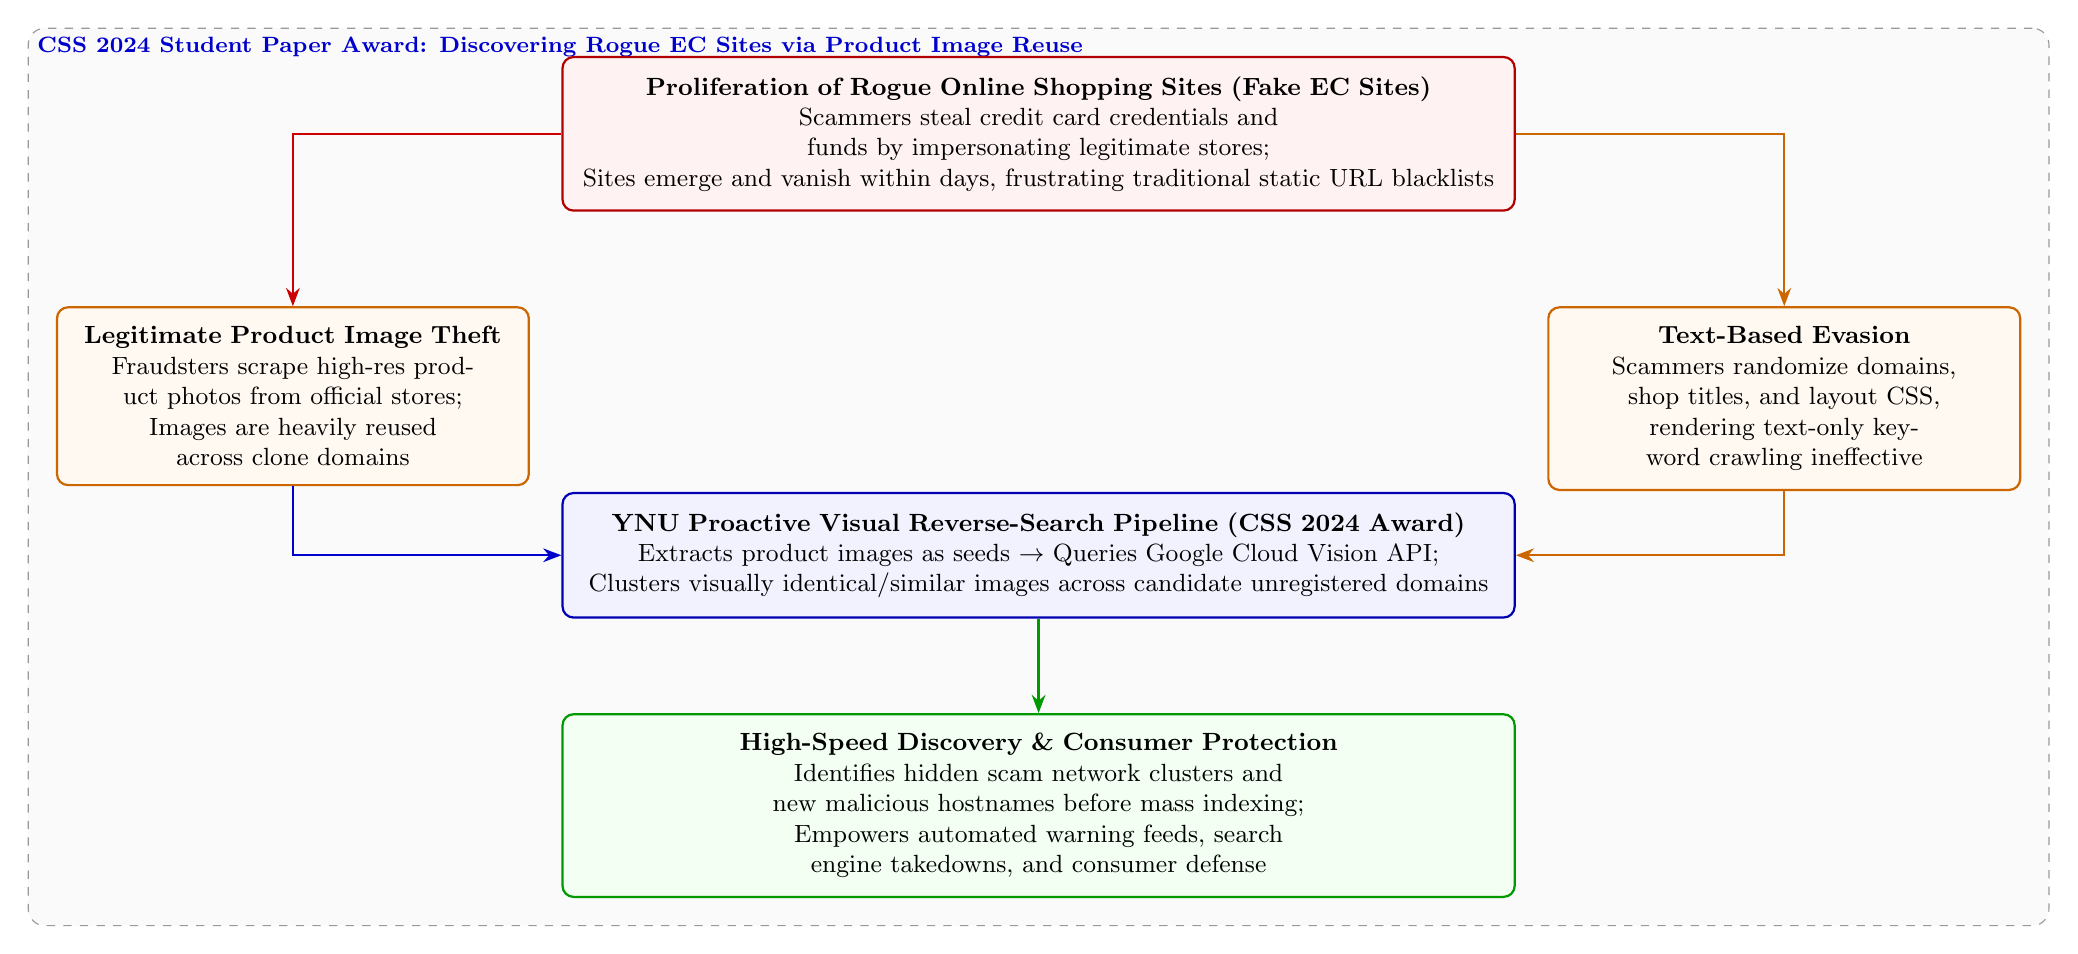
\begin{tikzpicture}[
    font=\small,
    >=Stealth,
    node distance=1.2cm,
    block/.style={rectangle, draw=blue!70!black, fill=blue!5, rounded corners=4pt, thick, align=center, inner sep=7pt},
    alertblock/.style={rectangle, draw=red!70!black, fill=red!5, rounded corners=4pt, thick, align=center, inner sep=7pt},
    greenblock/.style={rectangle, draw=green!60!black, fill=green!5, rounded corners=4pt, thick, align=center, inner sep=7pt},
    amberblock/.style={rectangle, draw=orange!80!black, fill=orange!5, rounded corners=4pt, thick, align=center, inner sep=7pt},
    groupbox/.style={draw=black!40, dashed, rounded corners=6pt, fill=black!2, inner sep=10pt}
]

    % Top: Fraudulent Ecosystem
    \node[alertblock, text width=11.6cm] (fraud) {\textbf{Proliferation of Rogue Online Shopping Sites (Fake EC Sites)}\\Scammers steal credit card credentials and funds by impersonating legitimate stores;\\Sites emerge and vanish within days, frustrating traditional static URL blacklists};

    % Left: Root Cause (Image Scraping)
    \node[amberblock, below left=1.2cm and 0.4cm of fraud, text width=5.5cm] (scrape) {\textbf{Legitimate Product Image Theft}\\Fraudsters scrape high-res product photos from official stores;\\Images are heavily reused across clone domains};

    % Right: Blind Spot in Text Search
    \node[amberblock, below right=1.2cm and 0.4cm of fraud, text width=5.5cm] (blindspot) {\textbf{Text-Based Evasion}\\Scammers randomize domains, shop titles, and layout CSS,\\rendering text-only keyword crawling ineffective};

    \draw[->, thick, red!80!black] (fraud) -| (scrape);
    \draw[->, thick, orange!80!black] (fraud) -| (blindspot);

    % Middle: Proposed Reverse Visual Pipeline
    \node[block, below=1.2cm of $(scrape)!0.5!(blindspot)$, text width=11.6cm] (vision) {\textbf{YNU Proactive Visual Reverse-Search Pipeline (CSS 2024 Award)}\\Extracts product images as seeds $\rightarrow$ Queries Google Cloud Vision API;\\Clusters visually identical/similar images across candidate unregistered domains};

    \draw[->, thick, blue!80!black] (scrape) |- (vision);
    \draw[->, thick, orange!80!black] (blindspot) |- (vision);

    % Bottom: Outcome
    \node[greenblock, below=1.2cm of vision, text width=11.6cm] (impact) {\textbf{High-Speed Discovery \& Consumer Protection}\\Identifies hidden scam network clusters and new malicious hostnames before mass indexing;\\Empowers automated warning feeds, search engine takedowns, and consumer defense};

    \draw[->, thick, green!60!black] (vision) -- (impact);

    \begin{scope}[on background layer]
        \node[groupbox, fit=(fraud) (scrape) (blindspot) (vision) (impact), label={[anchor=north west, font=\footnotesize\bfseries, blue!80!black]north west:CSS 2024 Student Paper Award: Discovering Rogue EC Sites via Product Image Reuse}] {};
    \end{scope}

\end{tikzpicture}
\end{document}
